% Options for packages loaded elsewhere
\PassOptionsToPackage{unicode}{hyperref}
\PassOptionsToPackage{hyphens}{url}
%
\documentclass[
]{article}
\title{STAT641\_FINAL\_REPORT}
\author{Abbas Jalili}
\date{2/28/2022}

\usepackage{amsmath,amssymb}
\usepackage{lmodern}
\usepackage{iftex}
\ifPDFTeX
  \usepackage[T1]{fontenc}
  \usepackage[utf8]{inputenc}
  \usepackage{textcomp} % provide euro and other symbols
\else % if luatex or xetex
  \usepackage{unicode-math}
  \defaultfontfeatures{Scale=MatchLowercase}
  \defaultfontfeatures[\rmfamily]{Ligatures=TeX,Scale=1}
\fi
% Use upquote if available, for straight quotes in verbatim environments
\IfFileExists{upquote.sty}{\usepackage{upquote}}{}
\IfFileExists{microtype.sty}{% use microtype if available
  \usepackage[]{microtype}
  \UseMicrotypeSet[protrusion]{basicmath} % disable protrusion for tt fonts
}{}
\makeatletter
\@ifundefined{KOMAClassName}{% if non-KOMA class
  \IfFileExists{parskip.sty}{%
    \usepackage{parskip}
  }{% else
    \setlength{\parindent}{0pt}
    \setlength{\parskip}{6pt plus 2pt minus 1pt}}
}{% if KOMA class
  \KOMAoptions{parskip=half}}
\makeatother
\usepackage{xcolor}
\IfFileExists{xurl.sty}{\usepackage{xurl}}{} % add URL line breaks if available
\IfFileExists{bookmark.sty}{\usepackage{bookmark}}{\usepackage{hyperref}}
\hypersetup{
  pdftitle={STAT641\_FINAL\_REPORT},
  pdfauthor={Abbas Jalili},
  hidelinks,
  pdfcreator={LaTeX via pandoc}}
\urlstyle{same} % disable monospaced font for URLs
\usepackage[margin=1in]{geometry}
\usepackage{color}
\usepackage{fancyvrb}
\newcommand{\VerbBar}{|}
\newcommand{\VERB}{\Verb[commandchars=\\\{\}]}
\DefineVerbatimEnvironment{Highlighting}{Verbatim}{commandchars=\\\{\}}
% Add ',fontsize=\small' for more characters per line
\usepackage{framed}
\definecolor{shadecolor}{RGB}{248,248,248}
\newenvironment{Shaded}{\begin{snugshade}}{\end{snugshade}}
\newcommand{\AlertTok}[1]{\textcolor[rgb]{0.94,0.16,0.16}{#1}}
\newcommand{\AnnotationTok}[1]{\textcolor[rgb]{0.56,0.35,0.01}{\textbf{\textit{#1}}}}
\newcommand{\AttributeTok}[1]{\textcolor[rgb]{0.77,0.63,0.00}{#1}}
\newcommand{\BaseNTok}[1]{\textcolor[rgb]{0.00,0.00,0.81}{#1}}
\newcommand{\BuiltInTok}[1]{#1}
\newcommand{\CharTok}[1]{\textcolor[rgb]{0.31,0.60,0.02}{#1}}
\newcommand{\CommentTok}[1]{\textcolor[rgb]{0.56,0.35,0.01}{\textit{#1}}}
\newcommand{\CommentVarTok}[1]{\textcolor[rgb]{0.56,0.35,0.01}{\textbf{\textit{#1}}}}
\newcommand{\ConstantTok}[1]{\textcolor[rgb]{0.00,0.00,0.00}{#1}}
\newcommand{\ControlFlowTok}[1]{\textcolor[rgb]{0.13,0.29,0.53}{\textbf{#1}}}
\newcommand{\DataTypeTok}[1]{\textcolor[rgb]{0.13,0.29,0.53}{#1}}
\newcommand{\DecValTok}[1]{\textcolor[rgb]{0.00,0.00,0.81}{#1}}
\newcommand{\DocumentationTok}[1]{\textcolor[rgb]{0.56,0.35,0.01}{\textbf{\textit{#1}}}}
\newcommand{\ErrorTok}[1]{\textcolor[rgb]{0.64,0.00,0.00}{\textbf{#1}}}
\newcommand{\ExtensionTok}[1]{#1}
\newcommand{\FloatTok}[1]{\textcolor[rgb]{0.00,0.00,0.81}{#1}}
\newcommand{\FunctionTok}[1]{\textcolor[rgb]{0.00,0.00,0.00}{#1}}
\newcommand{\ImportTok}[1]{#1}
\newcommand{\InformationTok}[1]{\textcolor[rgb]{0.56,0.35,0.01}{\textbf{\textit{#1}}}}
\newcommand{\KeywordTok}[1]{\textcolor[rgb]{0.13,0.29,0.53}{\textbf{#1}}}
\newcommand{\NormalTok}[1]{#1}
\newcommand{\OperatorTok}[1]{\textcolor[rgb]{0.81,0.36,0.00}{\textbf{#1}}}
\newcommand{\OtherTok}[1]{\textcolor[rgb]{0.56,0.35,0.01}{#1}}
\newcommand{\PreprocessorTok}[1]{\textcolor[rgb]{0.56,0.35,0.01}{\textit{#1}}}
\newcommand{\RegionMarkerTok}[1]{#1}
\newcommand{\SpecialCharTok}[1]{\textcolor[rgb]{0.00,0.00,0.00}{#1}}
\newcommand{\SpecialStringTok}[1]{\textcolor[rgb]{0.31,0.60,0.02}{#1}}
\newcommand{\StringTok}[1]{\textcolor[rgb]{0.31,0.60,0.02}{#1}}
\newcommand{\VariableTok}[1]{\textcolor[rgb]{0.00,0.00,0.00}{#1}}
\newcommand{\VerbatimStringTok}[1]{\textcolor[rgb]{0.31,0.60,0.02}{#1}}
\newcommand{\WarningTok}[1]{\textcolor[rgb]{0.56,0.35,0.01}{\textbf{\textit{#1}}}}
\usepackage{graphicx}
\makeatletter
\def\maxwidth{\ifdim\Gin@nat@width>\linewidth\linewidth\else\Gin@nat@width\fi}
\def\maxheight{\ifdim\Gin@nat@height>\textheight\textheight\else\Gin@nat@height\fi}
\makeatother
% Scale images if necessary, so that they will not overflow the page
% margins by default, and it is still possible to overwrite the defaults
% using explicit options in \includegraphics[width, height, ...]{}
\setkeys{Gin}{width=\maxwidth,height=\maxheight,keepaspectratio}
% Set default figure placement to htbp
\makeatletter
\def\fps@figure{htbp}
\makeatother
\setlength{\emergencystretch}{3em} % prevent overfull lines
\providecommand{\tightlist}{%
  \setlength{\itemsep}{0pt}\setlength{\parskip}{0pt}}
\setcounter{secnumdepth}{-\maxdimen} % remove section numbering
\ifLuaTeX
  \usepackage{selnolig}  % disable illegal ligatures
\fi

\begin{document}
\maketitle

\begin{Shaded}
\begin{Highlighting}[]
\NormalTok{pacman}\SpecialCharTok{::}\FunctionTok{p\_load}\NormalTok{(boot, tidyverse, infer)}
\end{Highlighting}
\end{Shaded}

\begin{Shaded}
\begin{Highlighting}[]
\NormalTok{body\_fat }\OtherTok{\textless{}{-}} \FunctionTok{read.csv}\NormalTok{(}\StringTok{"C:/Users/AJALI/Downloads/Compressed/archive\_2/bodyfat.csv"}\NormalTok{)}
\FunctionTok{head}\NormalTok{(body\_fat, }\DecValTok{5}\NormalTok{)}
\end{Highlighting}
\end{Shaded}

\begin{verbatim}
##   Density BodyFat Age Weight Height Neck Chest Abdomen   Hip Thigh Knee Ankle
## 1  1.0708    12.3  23 154.25  67.75 36.2  93.1    85.2  94.5  59.0 37.3  21.9
## 2  1.0853     6.1  22 173.25  72.25 38.5  93.6    83.0  98.7  58.7 37.3  23.4
## 3  1.0414    25.3  22 154.00  66.25 34.0  95.8    87.9  99.2  59.6 38.9  24.0
## 4  1.0751    10.4  26 184.75  72.25 37.4 101.8    86.4 101.2  60.1 37.3  22.8
## 5  1.0340    28.7  24 184.25  71.25 34.4  97.3   100.0 101.9  63.2 42.2  24.0
##   Biceps Forearm Wrist
## 1   32.0    27.4  17.1
## 2   30.5    28.9  18.2
## 3   28.8    25.2  16.6
## 4   32.4    29.4  18.2
## 5   32.2    27.7  17.7
\end{verbatim}

\begin{Shaded}
\begin{Highlighting}[]
\FunctionTok{max}\NormalTok{(body\_fat}\SpecialCharTok{$}\NormalTok{Age)}
\end{Highlighting}
\end{Shaded}

\begin{verbatim}
## [1] 81
\end{verbatim}

\begin{Shaded}
\begin{Highlighting}[]
\FunctionTok{min}\NormalTok{(body\_fat}\SpecialCharTok{$}\NormalTok{Age)}
\end{Highlighting}
\end{Shaded}

\begin{verbatim}
## [1] 22
\end{verbatim}

\begin{Shaded}
\begin{Highlighting}[]
\FunctionTok{dim}\NormalTok{(body\_fat)}
\end{Highlighting}
\end{Shaded}

\begin{verbatim}
## [1] 252  15
\end{verbatim}

\begin{Shaded}
\begin{Highlighting}[]
\FunctionTok{sum}\NormalTok{(}\FunctionTok{is.na}\NormalTok{(body\_fat))}
\end{Highlighting}
\end{Shaded}

\begin{verbatim}
## [1] 0
\end{verbatim}

\newpage

\begin{Shaded}
\begin{Highlighting}[]
\FunctionTok{set.seed}\NormalTok{(}\DecValTok{123}\NormalTok{)}
\NormalTok{body\_model }\OtherTok{\textless{}{-}} \FunctionTok{lm}\NormalTok{(Age }\SpecialCharTok{\textasciitilde{}}\NormalTok{ Weight}\SpecialCharTok{+}\NormalTok{Height}\SpecialCharTok{+}\NormalTok{Density}\SpecialCharTok{+}\NormalTok{Neck}\SpecialCharTok{+}\NormalTok{Chest}\SpecialCharTok{+}\NormalTok{Abdomen}\SpecialCharTok{+}\NormalTok{Hip}\SpecialCharTok{+}\NormalTok{Thigh}\SpecialCharTok{+}\NormalTok{Knee}\SpecialCharTok{+}\NormalTok{Ankle}\SpecialCharTok{+}
\NormalTok{                   Biceps}\SpecialCharTok{+}\NormalTok{Forearm}\SpecialCharTok{+}\NormalTok{Wrist}\SpecialCharTok{+}\NormalTok{ BodyFat,}\AttributeTok{data =}\NormalTok{ body\_fat)}
\FunctionTok{summary}\NormalTok{(body\_model)}
\end{Highlighting}
\end{Shaded}

\begin{verbatim}
## 
## Call:
## lm(formula = Age ~ Weight + Height + Density + Neck + Chest + 
##     Abdomen + Hip + Thigh + Knee + Ankle + Biceps + Forearm + 
##     Wrist + BodyFat, data = body_fat)
## 
## Residuals:
##      Min       1Q   Median       3Q      Max 
## -22.2848  -5.4626   0.1289   5.7231  23.4432 
## 
## Coefficients:
##               Estimate Std. Error t value Pr(>|t|)    
## (Intercept) -177.45849  209.00887  -0.849 0.396712    
## Weight        -0.32166    0.10539  -3.052 0.002531 ** 
## Height        -0.37010    0.18976  -1.950 0.052315 .  
## Density      146.06427  187.75564   0.778 0.437375    
## Neck           0.75398    0.46406   1.625 0.105546    
## Chest          0.09976    0.19767   0.505 0.614253    
## Abdomen        0.97212    0.20410   4.763 3.32e-06 ***
## Hip           -0.31695    0.29138  -1.088 0.277812    
## Thigh         -1.64799    0.26888  -6.129 3.66e-09 ***
## Knee           1.84321    0.46645   3.952 0.000103 ***
## Ankle         -0.70695    0.44133  -1.602 0.110523    
## Biceps         0.35701    0.34211   1.044 0.297758    
## Forearm       -1.09586    0.39419  -2.780 0.005872 ** 
## Wrist          5.85616    1.01834   5.751 2.73e-08 ***
## BodyFat        0.56903    0.43518   1.308 0.192288    
## ---
## Signif. codes:  0 '***' 0.001 '**' 0.01 '*' 0.05 '.' 0.1 ' ' 1
## 
## Residual standard error: 8.568 on 237 degrees of freedom
## Multiple R-squared:  0.5635, Adjusted R-squared:  0.5377 
## F-statistic: 21.86 on 14 and 237 DF,  p-value: < 2.2e-16
\end{verbatim}

\begin{Shaded}
\begin{Highlighting}[]
\CommentTok{\#making the null and full model fo anova:}
\NormalTok{null\_model }\OtherTok{\textless{}{-}} \FunctionTok{lm}\NormalTok{(Age }\SpecialCharTok{\textasciitilde{}} \DecValTok{1}\NormalTok{, }\AttributeTok{data =}\NormalTok{ body\_fat)}
\NormalTok{full\_model }\OtherTok{\textless{}{-}} \FunctionTok{lm}\NormalTok{(Age }\SpecialCharTok{\textasciitilde{}}\NormalTok{ ., }\AttributeTok{data =}\NormalTok{ body\_fat)}
\CommentTok{\# Comparing a full model with all the predictors to the null model or an initial model.}
\FunctionTok{anova}\NormalTok{(null\_model, full\_model)}
\end{Highlighting}
\end{Shaded}

\begin{verbatim}
## Analysis of Variance Table
## 
## Model 1: Age ~ 1
## Model 2: Age ~ Density + BodyFat + Weight + Height + Neck + Chest + Abdomen + 
##     Hip + Thigh + Knee + Ankle + Biceps + Forearm + Wrist
##   Res.Df   RSS Df Sum of Sq      F    Pr(>F)    
## 1    251 39862                                  
## 2    237 17398 14     22463 21.857 < 2.2e-16 ***
## ---
## Signif. codes:  0 '***' 0.001 '**' 0.01 '*' 0.05 '.' 0.1 ' ' 1
\end{verbatim}

\begin{Shaded}
\begin{Highlighting}[]
\CommentTok{\# Use a stepwise selection method.}
\FunctionTok{step}\NormalTok{(full\_model, }\AttributeTok{scope =} \FunctionTok{list}\NormalTok{(}\AttributeTok{lower =}\NormalTok{ null\_model, }\AttributeTok{upper =}\NormalTok{ full\_model), }\AttributeTok{trace =} \DecValTok{0}\NormalTok{)}
\end{Highlighting}
\end{Shaded}

\begin{verbatim}
## 
## Call:
## lm(formula = Age ~ BodyFat + Weight + Height + Neck + Abdomen + 
##     Thigh + Knee + Ankle + Forearm + Wrist, data = body_fat)
## 
## Coefficients:
## (Intercept)      BodyFat       Weight       Height         Neck      Abdomen  
##    -27.9872       0.2724      -0.3322      -0.3597       0.9427       0.9344  
##       Thigh         Knee        Ankle      Forearm        Wrist  
##     -1.7646       1.7613      -0.7560      -0.8997       6.0410
\end{verbatim}

\begin{Shaded}
\begin{Highlighting}[]
\CommentTok{\#fitting the model after stepwise model selection:}
\FunctionTok{set.seed}\NormalTok{(}\DecValTok{123}\NormalTok{)}
\NormalTok{new\_model }\OtherTok{\textless{}{-}} \FunctionTok{lm}\NormalTok{(Age }\SpecialCharTok{\textasciitilde{}}\NormalTok{ BodyFat }\SpecialCharTok{+}\NormalTok{ Weight }\SpecialCharTok{+}\NormalTok{ Height }\SpecialCharTok{+}\NormalTok{ Neck }\SpecialCharTok{+}\NormalTok{ Abdomen }\SpecialCharTok{+}\NormalTok{ Thigh }\SpecialCharTok{+}\NormalTok{ Knee }\SpecialCharTok{+}\NormalTok{ Ankle }\SpecialCharTok{+} 
\NormalTok{                  Forearm }\SpecialCharTok{+}\NormalTok{ Wrist, }\AttributeTok{data =}\NormalTok{ body\_fat)}
\FunctionTok{summary}\NormalTok{(new\_model)}
\end{Highlighting}
\end{Shaded}

\begin{verbatim}
## 
## Call:
## lm(formula = Age ~ BodyFat + Weight + Height + Neck + Abdomen + 
##     Thigh + Knee + Ankle + Forearm + Wrist, data = body_fat)
## 
## Residuals:
##      Min       1Q   Median       3Q      Max 
## -22.4793  -5.2087   0.1831   5.7306  23.5096 
## 
## Coefficients:
##              Estimate Std. Error t value Pr(>|t|)    
## (Intercept) -27.98721   25.32593  -1.105 0.270226    
## BodyFat       0.27240    0.12676   2.149 0.032642 *  
## Weight       -0.33216    0.07969  -4.168 4.29e-05 ***
## Height       -0.35967    0.18018  -1.996 0.047039 *  
## Neck          0.94272    0.45030   2.094 0.037345 *  
## Abdomen       0.93441    0.17905   5.219 3.89e-07 ***
## Thigh        -1.76456    0.23121  -7.632 5.38e-13 ***
## Knee          1.76132    0.46276   3.806 0.000179 ***
## Ankle        -0.75604    0.43736  -1.729 0.085156 .  
## Forearm      -0.89971    0.37169  -2.421 0.016237 *  
## Wrist         6.04102    1.01009   5.981 7.97e-09 ***
## ---
## Signif. codes:  0 '***' 0.001 '**' 0.01 '*' 0.05 '.' 0.1 ' ' 1
## 
## Residual standard error: 8.561 on 241 degrees of freedom
## Multiple R-squared:  0.5569, Adjusted R-squared:  0.5385 
## F-statistic: 30.29 on 10 and 241 DF,  p-value: < 2.2e-16
\end{verbatim}

\begin{Shaded}
\begin{Highlighting}[]
\FunctionTok{par}\NormalTok{(}\AttributeTok{mfrow =} \FunctionTok{c}\NormalTok{(}\DecValTok{1}\NormalTok{,}\DecValTok{2}\NormalTok{))}
\FunctionTok{plot}\NormalTok{(new\_model, }\AttributeTok{index =} \DecValTok{1}\NormalTok{)}
\end{Highlighting}
\end{Shaded}

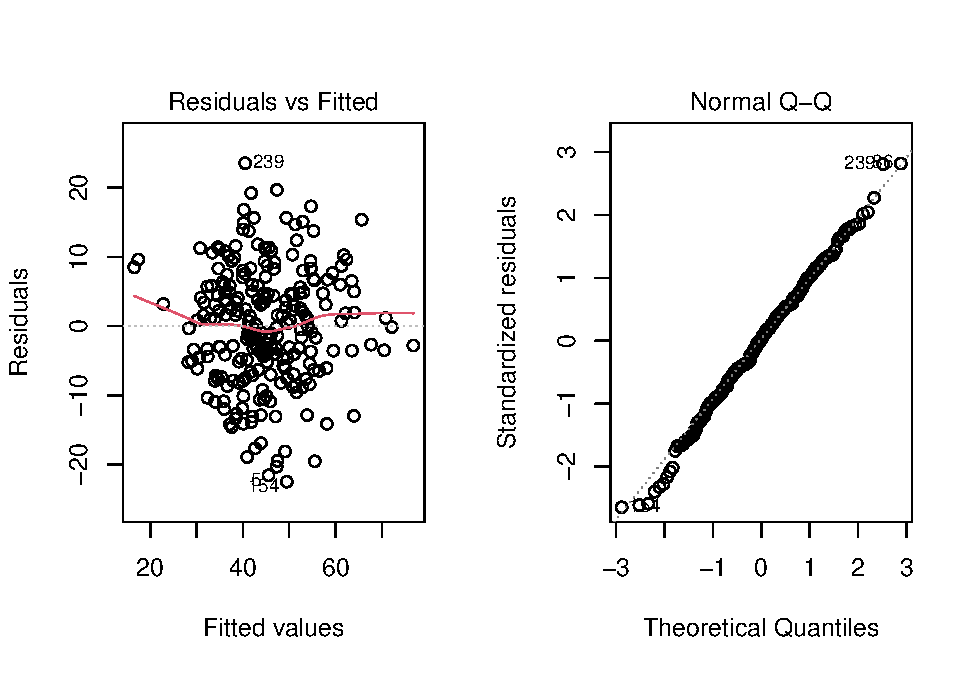
\includegraphics{STAT641_Final_Report_files/figure-latex/unnamed-chunk-7-1.pdf}
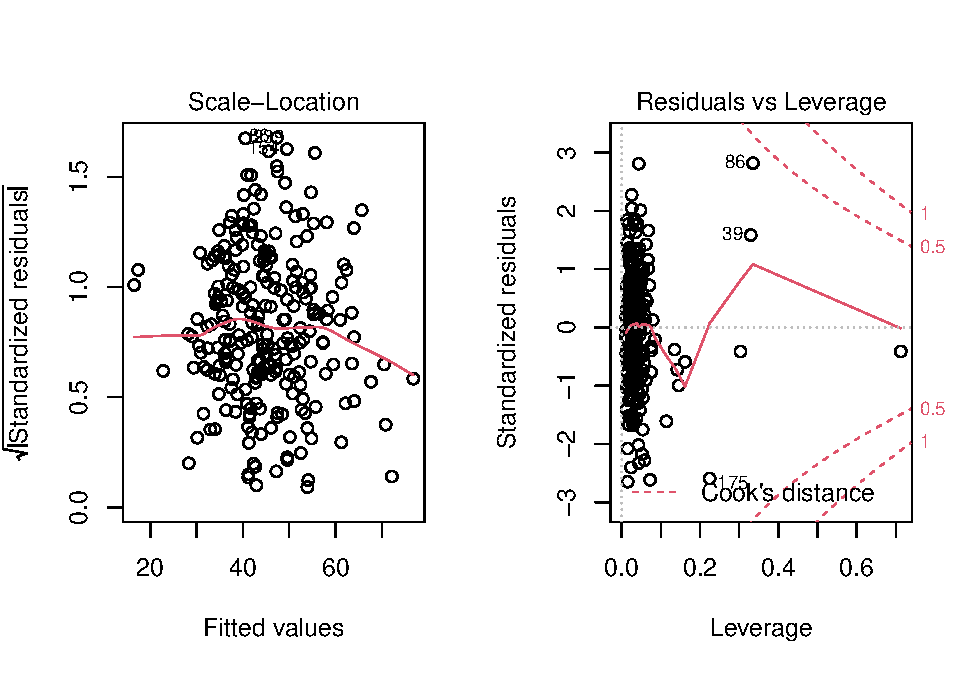
\includegraphics{STAT641_Final_Report_files/figure-latex/unnamed-chunk-7-2.pdf}

\neapage

\begin{Shaded}
\begin{Highlighting}[]
\FunctionTok{set.seed}\NormalTok{(}\DecValTok{123}\NormalTok{)}
\CommentTok{\#residual bootstrap resampling(fixed X):}
\NormalTok{fit\_body }\OtherTok{\textless{}{-}} \FunctionTok{fitted}\NormalTok{(new\_model)}
\NormalTok{e\_body }\OtherTok{\textless{}{-}} \FunctionTok{residuals}\NormalTok{(new\_model)}
\NormalTok{X\_body }\OtherTok{\textless{}{-}} \FunctionTok{model.matrix}\NormalTok{(new\_model)}

\NormalTok{boot.fixed\_body }\OtherTok{\textless{}{-}} \ControlFlowTok{function}\NormalTok{(data, i)\{}
\NormalTok{  y\_body }\OtherTok{\textless{}{-}}\NormalTok{ fit\_body }\SpecialCharTok{+}\NormalTok{ e\_body[i]}
\NormalTok{  mod\_body }\OtherTok{\textless{}{-}} \FunctionTok{lm}\NormalTok{(y\_body }\SpecialCharTok{\textasciitilde{}}\NormalTok{ X\_body }\SpecialCharTok{{-}} \DecValTok{1}\NormalTok{)}
  \FunctionTok{coefficients}\NormalTok{(mod\_body)}
\NormalTok{\}}
\NormalTok{body\_fixed\_boot }\OtherTok{\textless{}{-}} \FunctionTok{boot}\NormalTok{(body\_fat, boot.fixed\_body, }\DecValTok{5000}\NormalTok{)}
\NormalTok{body\_fixed\_boot}
\end{Highlighting}
\end{Shaded}

\begin{verbatim}
## 
## ORDINARY NONPARAMETRIC BOOTSTRAP
## 
## 
## Call:
## boot(data = body_fat, statistic = boot.fixed_body, R = 5000)
## 
## 
## Bootstrap Statistics :
##         original        bias    std. error
## t1*  -27.9872076  0.4119094186 25.20934737
## t2*    0.2723987 -0.0027860505  0.12379289
## t3*   -0.3321585  0.0009656434  0.07853564
## t4*   -0.3596654 -0.0028955306  0.17473208
## t5*    0.9427201  0.0037868682  0.43116909
## t6*    0.9344130  0.0029870094  0.17773945
## t7*   -1.7645638 -0.0026508901  0.22359025
## t8*    1.7613209 -0.0064416741  0.45841674
## t9*   -0.7560375  0.0036828213  0.42332464
## t10*  -0.8997090 -0.0001609307  0.35918134
## t11*   6.0410162 -0.0226273225  0.99493612
\end{verbatim}

\begin{Shaded}
\begin{Highlighting}[]
\FunctionTok{par}\NormalTok{(}\AttributeTok{mfrow =} \FunctionTok{c}\NormalTok{(}\DecValTok{1}\NormalTok{,}\DecValTok{2}\NormalTok{))}
\FunctionTok{plot}\NormalTok{(body\_fixed\_boot, }\AttributeTok{index =} \DecValTok{1}\NormalTok{)}
\end{Highlighting}
\end{Shaded}

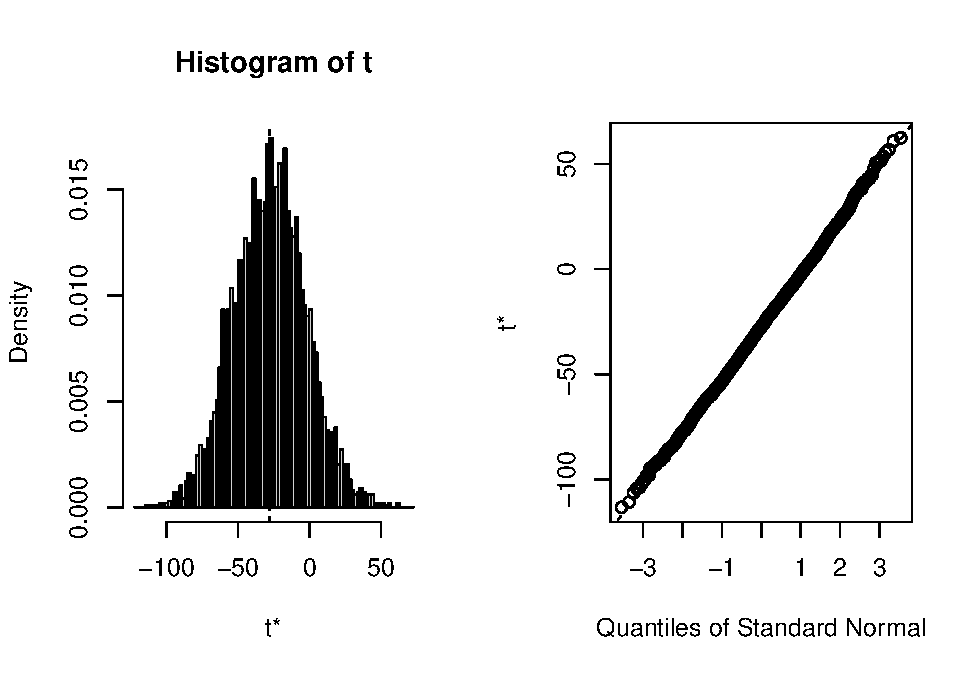
\includegraphics{STAT641_Final_Report_files/figure-latex/unnamed-chunk-9-1.pdf}

\begin{Shaded}
\begin{Highlighting}[]
\FunctionTok{par}\NormalTok{(}\AttributeTok{mfrow =} \FunctionTok{c}\NormalTok{(}\DecValTok{1}\NormalTok{,}\DecValTok{2}\NormalTok{))}
\FunctionTok{plot}\NormalTok{(body\_fixed\_boot, }\AttributeTok{index =} \DecValTok{2}\NormalTok{)}
\end{Highlighting}
\end{Shaded}

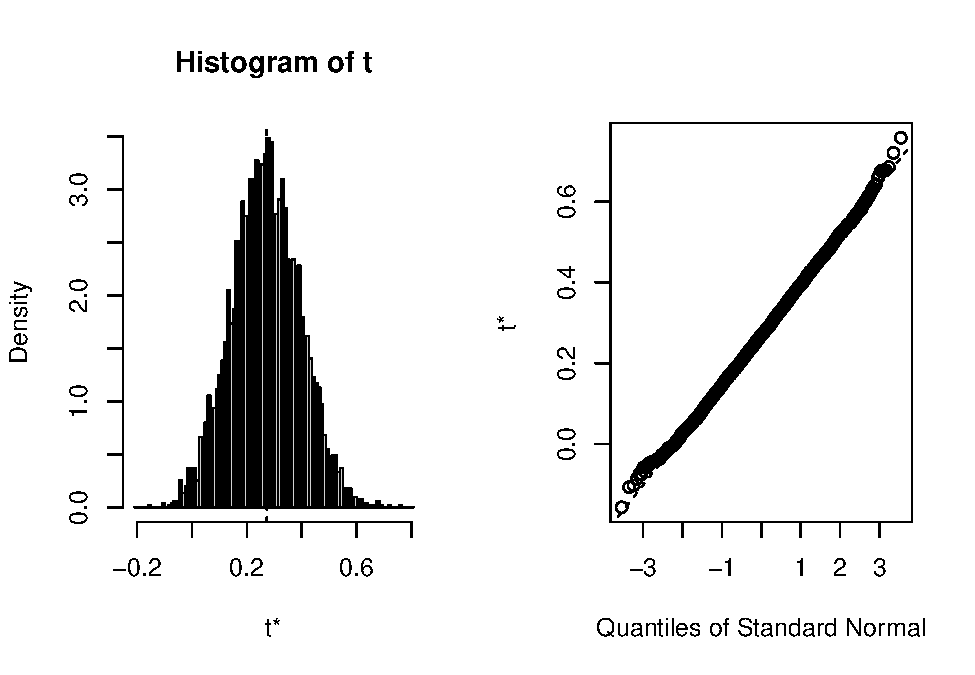
\includegraphics{STAT641_Final_Report_files/figure-latex/unnamed-chunk-10-1.pdf}

\begin{Shaded}
\begin{Highlighting}[]
\FunctionTok{par}\NormalTok{(}\AttributeTok{mfrow =} \FunctionTok{c}\NormalTok{(}\DecValTok{1}\NormalTok{,}\DecValTok{2}\NormalTok{))}
\FunctionTok{plot}\NormalTok{(body\_fixed\_boot, }\AttributeTok{index =} \DecValTok{3}\NormalTok{)}
\end{Highlighting}
\end{Shaded}

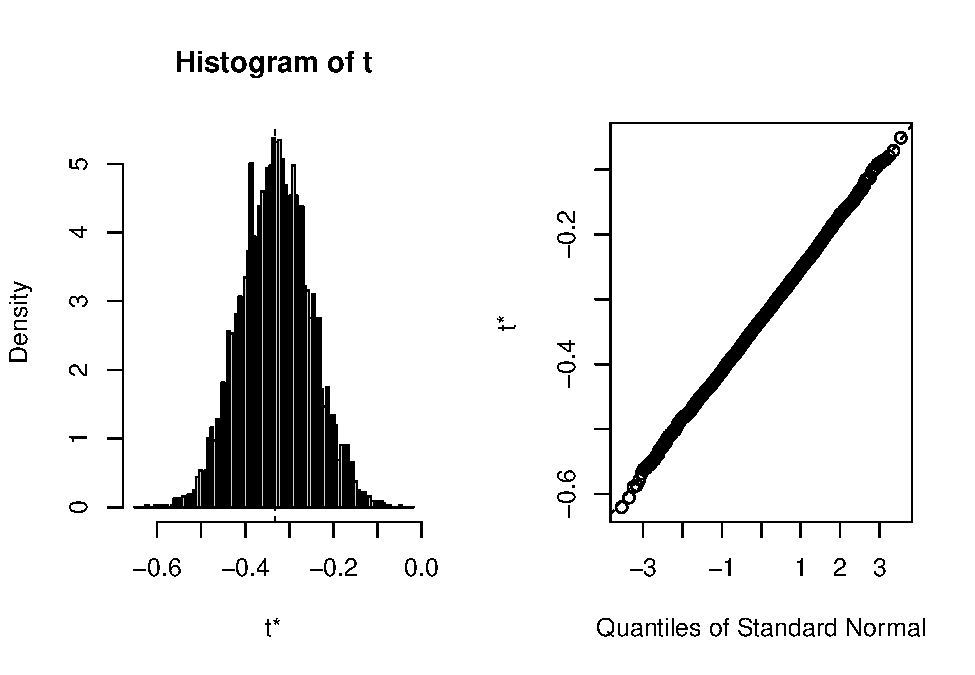
\includegraphics{STAT641_Final_Report_files/figure-latex/unnamed-chunk-11-1.pdf}

\begin{Shaded}
\begin{Highlighting}[]
\FunctionTok{par}\NormalTok{(}\AttributeTok{mfrow =} \FunctionTok{c}\NormalTok{(}\DecValTok{1}\NormalTok{,}\DecValTok{2}\NormalTok{))}
\FunctionTok{plot}\NormalTok{(body\_fixed\_boot, }\AttributeTok{index =} \DecValTok{4}\NormalTok{)}
\end{Highlighting}
\end{Shaded}

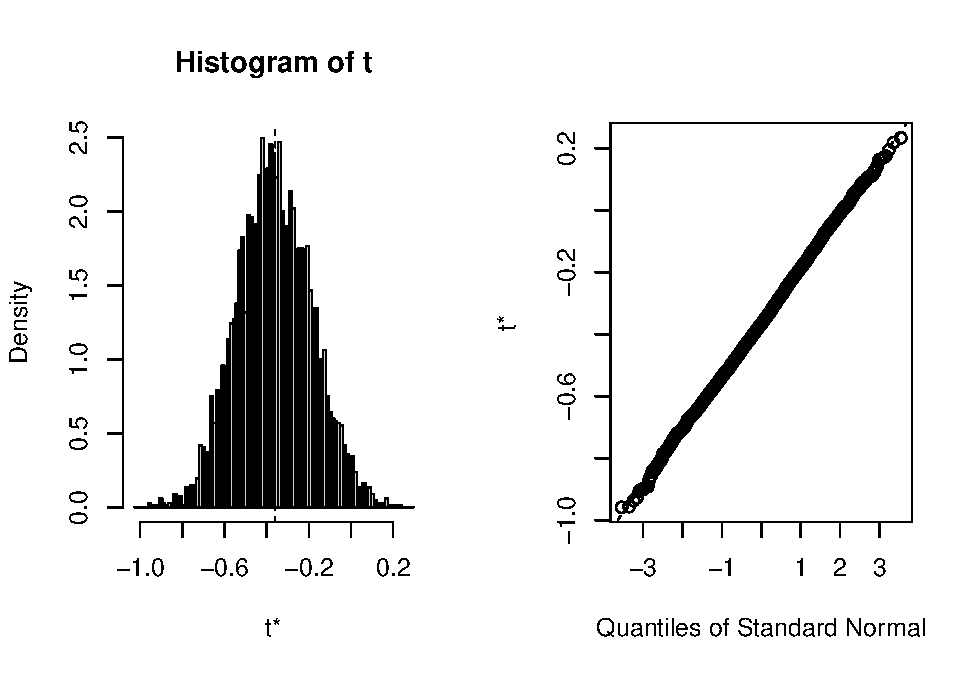
\includegraphics{STAT641_Final_Report_files/figure-latex/unnamed-chunk-12-1.pdf}

\begin{Shaded}
\begin{Highlighting}[]
\FunctionTok{set.seed}\NormalTok{(}\DecValTok{123}\NormalTok{)}
\NormalTok{boot.body }\OtherTok{\textless{}{-}} \ControlFlowTok{function}\NormalTok{(data, i)\{}
\NormalTok{  data }\OtherTok{\textless{}{-}}\NormalTok{ data[i,]}
\NormalTok{  model\_body }\OtherTok{\textless{}{-}} \FunctionTok{lm}\NormalTok{(Age }\SpecialCharTok{\textasciitilde{}}\NormalTok{ BodyFat }\SpecialCharTok{+}\NormalTok{ Weight }\SpecialCharTok{+}\NormalTok{ Height }\SpecialCharTok{+}\NormalTok{ Neck }\SpecialCharTok{+}\NormalTok{ Abdomen }\SpecialCharTok{+}\NormalTok{ Thigh }\SpecialCharTok{+} 
\NormalTok{                     Knee }\SpecialCharTok{+}\NormalTok{ Ankle }\SpecialCharTok{+}\NormalTok{ Forearm }\SpecialCharTok{+}\NormalTok{ Wrist,}\AttributeTok{data =}\NormalTok{ data)}
  \FunctionTok{coefficients}\NormalTok{(model\_body)}
\NormalTok{\}}

\NormalTok{model\_boot\_body }\OtherTok{\textless{}{-}} \FunctionTok{boot}\NormalTok{(body\_fat, boot.body, }\DecValTok{5000}\NormalTok{)}
\NormalTok{model\_boot\_body}
\end{Highlighting}
\end{Shaded}

\begin{verbatim}
## 
## ORDINARY NONPARAMETRIC BOOTSTRAP
## 
## 
## Call:
## boot(data = body_fat, statistic = boot.body, R = 5000)
## 
## 
## Bootstrap Statistics :
##         original       bias    std. error
## t1*  -27.9872076  2.373803686 28.28336557
## t2*    0.2723987  0.001326545  0.12238873
## t3*   -0.3321585  0.004402926  0.08832711
## t4*   -0.3596654 -0.014745298  0.23366021
## t5*    0.9427201 -0.051141811  0.46748994
## t6*    0.9344130 -0.010259643  0.16933894
## t7*   -1.7645638  0.016315230  0.23688076
## t8*    1.7613209  0.029031260  0.49994553
## t9*   -0.7560375 -0.187726802  0.71518077
## t10*  -0.8997090 -0.015257329  0.49710910
## t11*   6.0410162  0.188108013  1.00917611
\end{verbatim}

\begin{Shaded}
\begin{Highlighting}[]
\FunctionTok{par}\NormalTok{(}\AttributeTok{mfrow =} \FunctionTok{c}\NormalTok{(}\DecValTok{1}\NormalTok{,}\DecValTok{2}\NormalTok{))}
\FunctionTok{plot}\NormalTok{(model\_boot\_body, }\AttributeTok{index =} \DecValTok{1}\NormalTok{)}
\end{Highlighting}
\end{Shaded}

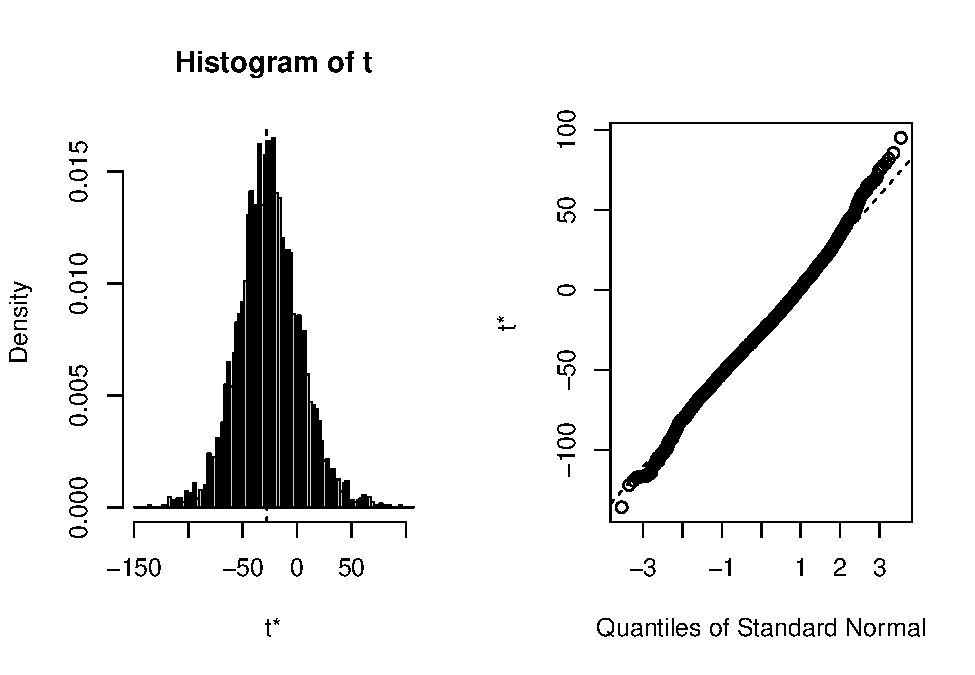
\includegraphics{STAT641_Final_Report_files/figure-latex/unnamed-chunk-14-1.pdf}

\begin{Shaded}
\begin{Highlighting}[]
\FunctionTok{par}\NormalTok{(}\AttributeTok{mfrow =} \FunctionTok{c}\NormalTok{(}\DecValTok{1}\NormalTok{,}\DecValTok{2}\NormalTok{))}
\FunctionTok{plot}\NormalTok{(model\_boot\_body, }\AttributeTok{index =} \DecValTok{2}\NormalTok{)}
\end{Highlighting}
\end{Shaded}

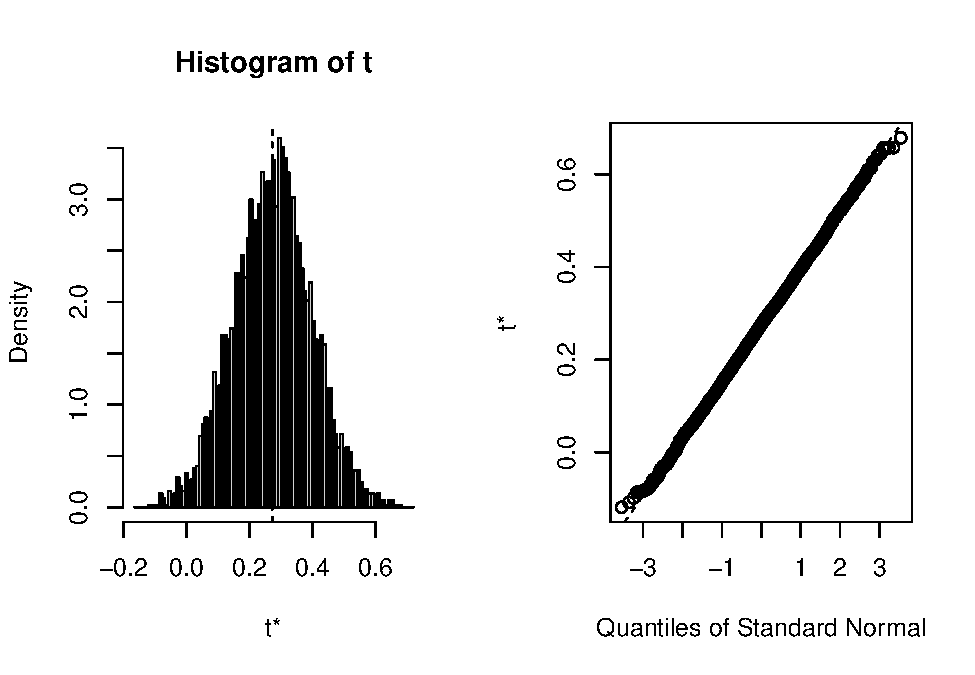
\includegraphics{STAT641_Final_Report_files/figure-latex/unnamed-chunk-15-1.pdf}

\begin{Shaded}
\begin{Highlighting}[]
\FunctionTok{par}\NormalTok{(}\AttributeTok{mfrow =} \FunctionTok{c}\NormalTok{(}\DecValTok{1}\NormalTok{,}\DecValTok{2}\NormalTok{))}
\FunctionTok{plot}\NormalTok{(model\_boot\_body, }\AttributeTok{index =} \DecValTok{3}\NormalTok{)}
\end{Highlighting}
\end{Shaded}

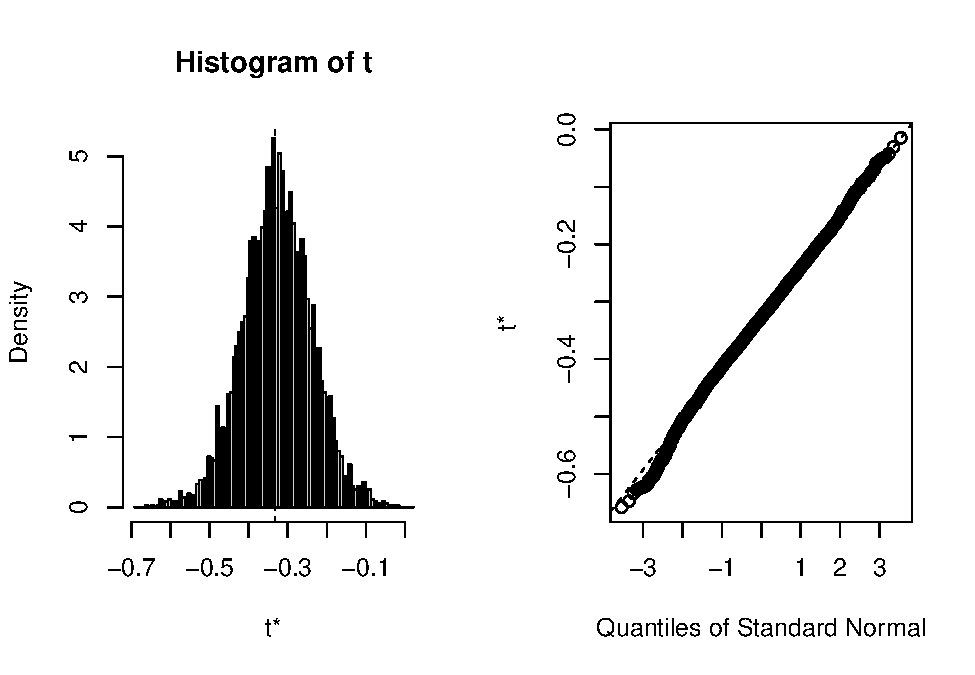
\includegraphics{STAT641_Final_Report_files/figure-latex/unnamed-chunk-16-1.pdf}

\begin{Shaded}
\begin{Highlighting}[]
\FunctionTok{par}\NormalTok{(}\AttributeTok{mfrow =} \FunctionTok{c}\NormalTok{(}\DecValTok{1}\NormalTok{,}\DecValTok{2}\NormalTok{))}
\FunctionTok{plot}\NormalTok{(model\_boot\_body, }\AttributeTok{index =} \DecValTok{4}\NormalTok{)}
\end{Highlighting}
\end{Shaded}

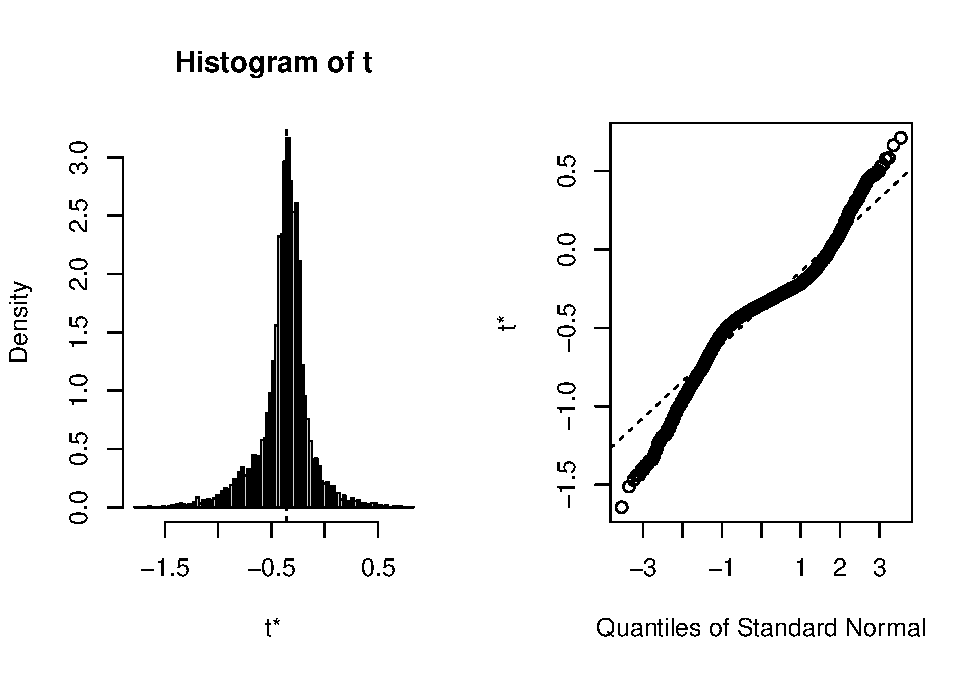
\includegraphics{STAT641_Final_Report_files/figure-latex/unnamed-chunk-17-1.pdf}

\begin{Shaded}
\begin{Highlighting}[]
\FunctionTok{boot.ci}\NormalTok{(model\_boot\_body, }\AttributeTok{index =} \DecValTok{1}\NormalTok{, }\AttributeTok{type =} \FunctionTok{c}\NormalTok{(}\StringTok{\textquotesingle{}norm\textquotesingle{}}\NormalTok{, }\StringTok{\textquotesingle{}perc\textquotesingle{}}\NormalTok{, }\StringTok{\textquotesingle{}bca\textquotesingle{}}\NormalTok{))}
\end{Highlighting}
\end{Shaded}

\begin{verbatim}
## BOOTSTRAP CONFIDENCE INTERVAL CALCULATIONS
## Based on 5000 bootstrap replicates
## 
## CALL : 
## boot.ci(boot.out = model_boot_body, type = c("norm", "perc", 
##     "bca"), index = 1)
## 
## Intervals : 
## Level      Normal             Percentile            BCa          
## 95%   (-85.80,  25.07 )   (-80.36,  32.78 )   (-84.51,  27.33 )  
## Calculations and Intervals on Original Scale
\end{verbatim}

\begin{Shaded}
\begin{Highlighting}[]
\FunctionTok{boot.ci}\NormalTok{(body\_fixed\_boot, }\AttributeTok{index =} \DecValTok{1}\NormalTok{, }\AttributeTok{type =} \FunctionTok{c}\NormalTok{(}\StringTok{\textquotesingle{}norm\textquotesingle{}}\NormalTok{, }\StringTok{\textquotesingle{}perc\textquotesingle{}}\NormalTok{, }\StringTok{\textquotesingle{}bca\textquotesingle{}}\NormalTok{))}
\end{Highlighting}
\end{Shaded}

\begin{verbatim}
## BOOTSTRAP CONFIDENCE INTERVAL CALCULATIONS
## Based on 5000 bootstrap replicates
## 
## CALL : 
## boot.ci(boot.out = body_fixed_boot, type = c("norm", "perc", 
##     "bca"), index = 1)
## 
## Intervals : 
## Level      Normal             Percentile            BCa          
## 95%   (-77.81,  21.01 )   (-76.91,  21.98 )   (-77.94,  21.26 )  
## Calculations and Intervals on Original Scale
\end{verbatim}

\begin{Shaded}
\begin{Highlighting}[]
\NormalTok{new\_bodyfat }\OtherTok{\textless{}{-}}\NormalTok{ body\_fat }\SpecialCharTok{\%\textgreater{}\%} \FunctionTok{mutate}\NormalTok{(}\AttributeTok{Group =} \FunctionTok{ifelse}\NormalTok{(Age}\SpecialCharTok{\textless{}=}\DecValTok{45}\NormalTok{, }\StringTok{"22{-}45"}\NormalTok{,}\StringTok{"46{-}81"}\NormalTok{))}
\FunctionTok{head}\NormalTok{(new\_bodyfat, }\DecValTok{5}\NormalTok{)}
\end{Highlighting}
\end{Shaded}

\begin{verbatim}
##   Density BodyFat Age Weight Height Neck Chest Abdomen   Hip Thigh Knee Ankle
## 1  1.0708    12.3  23 154.25  67.75 36.2  93.1    85.2  94.5  59.0 37.3  21.9
## 2  1.0853     6.1  22 173.25  72.25 38.5  93.6    83.0  98.7  58.7 37.3  23.4
## 3  1.0414    25.3  22 154.00  66.25 34.0  95.8    87.9  99.2  59.6 38.9  24.0
## 4  1.0751    10.4  26 184.75  72.25 37.4 101.8    86.4 101.2  60.1 37.3  22.8
## 5  1.0340    28.7  24 184.25  71.25 34.4  97.3   100.0 101.9  63.2 42.2  24.0
##   Biceps Forearm Wrist Group
## 1   32.0    27.4  17.1 22-45
## 2   30.5    28.9  18.2 22-45
## 3   28.8    25.2  16.6 22-45
## 4   32.4    29.4  18.2 22-45
## 5   32.2    27.7  17.7 22-45
\end{verbatim}

\begin{Shaded}
\begin{Highlighting}[]
\CommentTok{\# Visualize barplot using a ggplot2 package}
\NormalTok{new\_bodyfat }\SpecialCharTok{\%\textgreater{}\%}
  \FunctionTok{ggplot}\NormalTok{(}\FunctionTok{aes}\NormalTok{(}\AttributeTok{x =}\NormalTok{ Group, }\AttributeTok{fill =}\NormalTok{ Group)) }\SpecialCharTok{+} \FunctionTok{geom\_bar}\NormalTok{() }\SpecialCharTok{+} \FunctionTok{labs}\NormalTok{(}\AttributeTok{title =} \StringTok{"Age 22{-}45 Versus Age 46{-}81 Group"}\NormalTok{, }\AttributeTok{x =} \StringTok{"Groups"}\NormalTok{, }\AttributeTok{y =} \StringTok{"Count"}\NormalTok{) }\SpecialCharTok{+}\FunctionTok{theme}\NormalTok{(}\AttributeTok{panel.grid.major =} \FunctionTok{element\_blank}\NormalTok{())}
\end{Highlighting}
\end{Shaded}

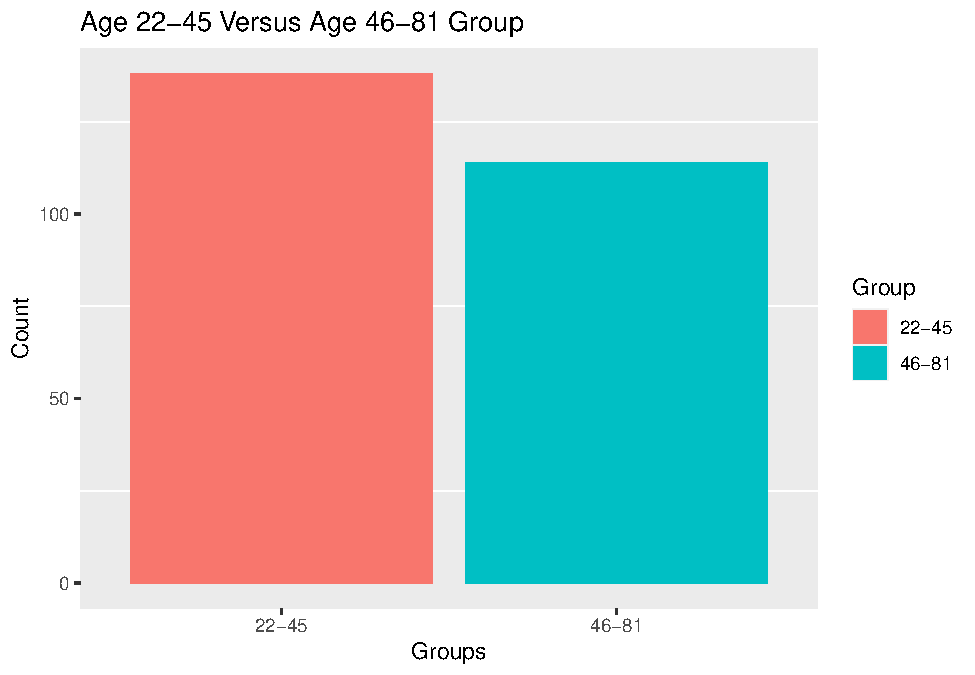
\includegraphics{STAT641_Final_Report_files/figure-latex/unnamed-chunk-21-1.pdf}

\begin{Shaded}
\begin{Highlighting}[]
\NormalTok{new\_df }\OtherTok{\textless{}{-}}\NormalTok{ new\_bodyfat }\SpecialCharTok{\%\textgreater{}\%} \FunctionTok{group\_by}\NormalTok{(Group)}\SpecialCharTok{\%\textgreater{}\%}
  \FunctionTok{summarise}\NormalTok{(}\AttributeTok{n =}\FunctionTok{n}\NormalTok{(),}
            \AttributeTok{Bodyfat\_mean =} \FunctionTok{mean}\NormalTok{(BodyFat))}
\NormalTok{new\_df}
\end{Highlighting}
\end{Shaded}

\begin{verbatim}
## # A tibble: 2 x 3
##   Group     n Bodyfat_mean
##   <chr> <int>        <dbl>
## 1 22-45   138         18.0
## 2 46-81   114         20.6
\end{verbatim}

\begin{Shaded}
\begin{Highlighting}[]
\FunctionTok{set.seed}\NormalTok{(}\DecValTok{123}\NormalTok{)}
\CommentTok{\# Calculate an observed test statistic.}
\NormalTok{obs\_test\_stat }\OtherTok{\textless{}{-}}\NormalTok{ new\_bodyfat }\SpecialCharTok{\%\textgreater{}\%}
  \FunctionTok{specify}\NormalTok{(BodyFat }\SpecialCharTok{\textasciitilde{}}\NormalTok{ Group)}\SpecialCharTok{\%\textgreater{}\%}
  \FunctionTok{calculate}\NormalTok{(}\AttributeTok{stat =} \StringTok{"diff in means"}\NormalTok{, }\AttributeTok{order =} \FunctionTok{c}\NormalTok{(}\StringTok{"46{-}81"}\NormalTok{,}\StringTok{"22{-}45"}\NormalTok{))}
\FunctionTok{round}\NormalTok{(obs\_test\_stat,}\DecValTok{2}\NormalTok{)}
\end{Highlighting}
\end{Shaded}

\begin{verbatim}
## Response: BodyFat (numeric)
## Explanatory: Group (factor)
## # A tibble: 1 x 1
##    stat
##   <dbl>
## 1  2.56
\end{verbatim}

\begin{Shaded}
\begin{Highlighting}[]
\CommentTok{\# To double check manually computed observed test statistics.}
\NormalTok{obs\_diff\_mean }\OtherTok{=} \FloatTok{20.55088} \SpecialCharTok{{-}}  \FloatTok{17.99420}     
\NormalTok{obs\_diff\_mean}
\end{Highlighting}
\end{Shaded}

\begin{verbatim}
## [1] 2.55668
\end{verbatim}

\begin{Shaded}
\begin{Highlighting}[]
\FunctionTok{set.seed}\NormalTok{(}\DecValTok{123}\NormalTok{)}
\CommentTok{\# Create the null distribution.}
\NormalTok{null\_dist }\OtherTok{\textless{}{-}}\NormalTok{ new\_bodyfat }\SpecialCharTok{\%\textgreater{}\%}
  \FunctionTok{specify}\NormalTok{(BodyFat }\SpecialCharTok{\textasciitilde{}}\NormalTok{ Group)}\SpecialCharTok{\%\textgreater{}\%}
  \FunctionTok{hypothesize}\NormalTok{(}\AttributeTok{null =} \StringTok{"independence"}\NormalTok{) }\SpecialCharTok{\%\textgreater{}\%}
  \FunctionTok{generate}\NormalTok{(}\AttributeTok{reps =} \DecValTok{5000}\NormalTok{, }\AttributeTok{type =} \StringTok{"permute"}\NormalTok{) }\SpecialCharTok{\%\textgreater{}\%}
  \FunctionTok{calculate}\NormalTok{(}\AttributeTok{stat =} \StringTok{"diff in means"}\NormalTok{, }\AttributeTok{order =} \FunctionTok{c}\NormalTok{(}\StringTok{"46{-}81"}\NormalTok{,}\StringTok{"22{-}45"}\NormalTok{))}
\FunctionTok{head}\NormalTok{(null\_dist,}\DecValTok{5}\NormalTok{)}
\end{Highlighting}
\end{Shaded}

\begin{verbatim}
## Response: BodyFat (numeric)
## Explanatory: Group (factor)
## Null Hypothesis: independence
## # A tibble: 5 x 2
##   replicate    stat
##       <int>   <dbl>
## 1         1  0.0834
## 2         2 -0.488 
## 3         3  0.162 
## 4         4  0.748 
## 5         5  1.47
\end{verbatim}

\begin{Shaded}
\begin{Highlighting}[]
\CommentTok{\# Visualize the null distribution.}
\NormalTok{null\_dist }\SpecialCharTok{\%\textgreater{}\%}
  \FunctionTok{visualize}\NormalTok{() }\SpecialCharTok{+}
  \FunctionTok{shade\_p\_value}\NormalTok{(}\AttributeTok{obs\_stat =}\NormalTok{ obs\_test\_stat, }\AttributeTok{direction =} \StringTok{"right"}\NormalTok{, }\AttributeTok{col =} \StringTok{"blue"}\NormalTok{, }\AttributeTok{lty =} \DecValTok{1}\NormalTok{, }\AttributeTok{lwd =} \DecValTok{1}\NormalTok{)}
\end{Highlighting}
\end{Shaded}

\begin{verbatim}
## Warning: Duplicated aesthetics after name standardisation: size
\end{verbatim}

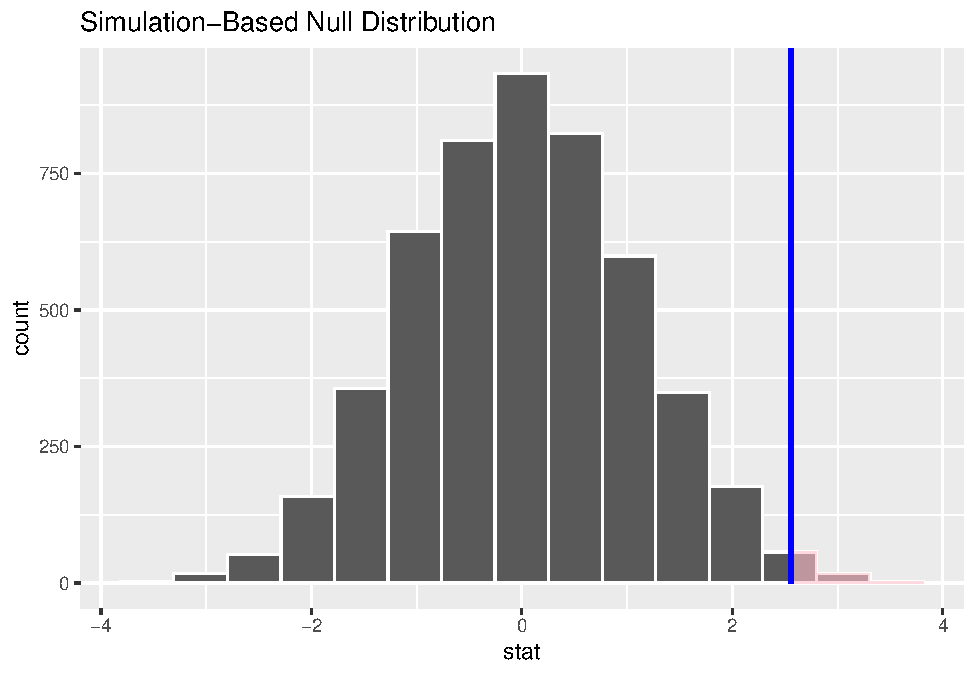
\includegraphics{STAT641_Final_Report_files/figure-latex/unnamed-chunk-24-1.pdf}

\begin{Shaded}
\begin{Highlighting}[]
\FunctionTok{set.seed}\NormalTok{(}\DecValTok{123}\NormalTok{)}
\CommentTok{\# Compute the p{-}value.}
\NormalTok{null\_dist }\SpecialCharTok{\%\textgreater{}\%}
  \FunctionTok{get\_p\_value}\NormalTok{(}\AttributeTok{obs\_stat =}\NormalTok{ obs\_test\_stat, }\AttributeTok{direction =} \StringTok{"right"}\NormalTok{)}
\end{Highlighting}
\end{Shaded}

\begin{verbatim}
## # A tibble: 1 x 1
##   p_value
##     <dbl>
## 1   0.007
\end{verbatim}

\end{document}
